\documentclass[]{article}
\usepackage{lmodern}
\usepackage{setspace}
\setstretch{2}
\usepackage{amssymb,amsmath}
\usepackage{ifxetex,ifluatex}
\usepackage{fixltx2e} % provides \textsubscript
\ifnum 0\ifxetex 1\fi\ifluatex 1\fi=0 % if pdftex
  \usepackage[T1]{fontenc}
  \usepackage[utf8]{inputenc}
\else % if luatex or xelatex
  \ifxetex
    \usepackage{mathspec}
  \else
    \usepackage{fontspec}
  \fi
  \defaultfontfeatures{Ligatures=TeX,Scale=MatchLowercase}
    \setmainfont[]{mathptmx}
\fi
% use upquote if available, for straight quotes in verbatim environments
\IfFileExists{upquote.sty}{\usepackage{upquote}}{}
% use microtype if available
\IfFileExists{microtype.sty}{%
\usepackage{microtype}
\UseMicrotypeSet[protrusion]{basicmath} % disable protrusion for tt fonts
}{}
\usepackage[margin=2.5cm]{geometry}
\usepackage{hyperref}
\hypersetup{unicode=true,
            pdfborder={0 0 0},
            breaklinks=true}
\urlstyle{same}  % don't use monospace font for urls
\usepackage{graphicx,grffile}
\makeatletter
\def\maxwidth{\ifdim\Gin@nat@width>\linewidth\linewidth\else\Gin@nat@width\fi}
\def\maxheight{\ifdim\Gin@nat@height>\textheight\textheight\else\Gin@nat@height\fi}
\makeatother
% Scale images if necessary, so that they will not overflow the page
% margins by default, and it is still possible to overwrite the defaults
% using explicit options in \includegraphics[width, height, ...]{}
\setkeys{Gin}{width=\maxwidth,height=\maxheight,keepaspectratio}
\IfFileExists{parskip.sty}{%
\usepackage{parskip}
}{% else
\setlength{\parindent}{0pt}
\setlength{\parskip}{6pt plus 2pt minus 1pt}
}
\setlength{\emergencystretch}{3em}  % prevent overfull lines
\providecommand{\tightlist}{%
  \setlength{\itemsep}{0pt}\setlength{\parskip}{0pt}}
\setcounter{secnumdepth}{0}
% Redefines (sub)paragraphs to behave more like sections
\ifx\paragraph\undefined\else
\let\oldparagraph\paragraph
\renewcommand{\paragraph}[1]{\oldparagraph{#1}\mbox{}}
\fi
\ifx\subparagraph\undefined\else
\let\oldsubparagraph\subparagraph
\renewcommand{\subparagraph}[1]{\oldsubparagraph{#1}\mbox{}}
\fi

%%% Use protect on footnotes to avoid problems with footnotes in titles
\let\rmarkdownfootnote\footnote%
\def\footnote{\protect\rmarkdownfootnote}

%%% Change title format to be more compact
\usepackage{titling}

% Create subtitle command for use in maketitle
\newcommand{\subtitle}[1]{
  \posttitle{
    \begin{center}\large#1\end{center}
    }
}

\setlength{\droptitle}{-2em}
  \title{}
  \pretitle{\vspace{\droptitle}}
  \posttitle{}
  \author{}
  \preauthor{}\postauthor{}
  \date{}
  \predate{}\postdate{}


\begin{document}

\pagebreak

TITLE \{-\}

Authors: Danielle C. Claar \(^1\), Kristina L. Tietjen \(^1\), Ruth D.
Gates \(^2\), Julia K. Baum \(^1\)

Institute: \(^1\) Department of Biology, University of Victoria, PO BOX
1700 Station CSC, Victoria, British Columbia, V8W 2Y2, Canada \(^2\)
Hawaii Institute of Marine Biology, 46-007 Lilipuna Road, Kaneohe, HI
96744, USA

Corresponding Author: Danielle C. Claar, Tel: (208) 250-0161, Email:
\href{mailto:dclaar@uvic.ca}{\nolinkurl{dclaar@uvic.ca}}

Keywords: coral bleaching, heat stress, climate change, Symbiodinium

\pagebreak 

\section*{Summary}\label{summary}
\addcontentsline{toc}{section}{Summary}

\emph{Let's leave this for now and come back to it once we have rest of
manuscript honed} Coral reefs, which already live on the edge of their
thermal tolerance\textsuperscript{1}, are under acute threat from ocean
warming\textsuperscript{2--4}. Corals live in symbiosis with an
extraordinarily diverse genus of photosynthetic dinoflagellates
(Symbiodinium spp.;\textsuperscript{5,6}). The symbiotic association and
diversity of various taxa of \emph{Symbiodinium} can be flexible over
time\textsuperscript{7,8}, but see\textsuperscript{9,10}, and individual
\emph{Symbidoinium} taxa can range from parasites to mutualists in their
interaction with their coral host\textsuperscript{11}. Warming causes
the breakdown of coral symbiosis, causing coral ``bleaching'' when
symbionts are expelled and the white coral skeleton is visible through
the coral tissue\textsuperscript{12}. Coral bleaching can lead to
mortality, although corals can regain their symbionts after heat stress
has abated\textsuperscript{13,14}. The 2015/16 El Niño is the worst
pulse warming event on record in terms of severity and
longevity\textsuperscript{{\textbf{???}},15}, yet despite massive coral
mortality, some corals show resilience to this extreme event
(\textbf{???}). Here, we track coral symbioses and survival at the
epicenter of this bleaching event (Kiritimati, Central Pacific), and
show, contrary to our current paradigm of coral bleaching and recovery
dynamics, that some corals have the capacity to re-establish symbiosis
before heat stress subsides. Furthermore, we demonstrate potential
mechanisms for coral survival and recovery, including the lack of
preferential symbiont expulsion, and the effect of local human
disturbance on pre-bleaching symbiont community structure and the
probability of coral survival. Together, these results show the
potential for reef corals to survive extreme warming events, providing
tentative hope for the survival of corals in the Anthropocene.

\pagebreak

\section*{Main Text}\label{main-text}
\addcontentsline{toc}{section}{Main Text}

NEED INTRO SENTENCE TO HOOK READERS. The symbiosis between coral and
their single-celled dinoflagellate symbionts, \emph{Symbiodinium}, is
the foundation of reef ecosystems, and a critical element of reef
resilience {[}16; Muller-Parker2015-sd{]}. The coral holobiont responds
to environmental conditions, and is the unit that interacts with the
broader reef community\textsuperscript{17}, supporting reef diversity
and function across taxa \emph{(or at a global scale?)}. There is much
genetic, functional, and response diversity within the
\emph{Symbiodinium} genus. Although \emph{Symbiodinium} is currently
classified as a single genus, it contains diversity similar to diversity
found within other dinoflagellate orders\textsuperscript{6}, and is
divided into nine clades and hundreds of types\textsuperscript{18--20}.
There is much debate about species classifications within
\emph{Symbiodinium}, which has hampered species naming within
\emph{Symbiodinium} {[}21; but see 22) although \emph{Symbiodinium}
types are generally considered putative species {[}23.
\emph{Symbiodinium} types have distinct geographic distributions, host
associations, and environmental optima\textsuperscript{24}. Furthermore,
total and relative abundance of \emph{Symbiodinium} can vary among coral
colonies, across environmental gradients, and over
time\textsuperscript{25}, with increased \emph{Symbiodinium} abundance
leading to increased environmental sensitivity and bleaching
risk\textsuperscript{26}. There are functional differences between
\emph{Symbiodinium} clades\textsuperscript{27}, and \emph{Symbiodinium}
associations can range from mutualistic to neutral to parasitic based on
\emph{Symbiodinium} type as well as environmental
conditions\textsuperscript{11}. Recent advances in next-generation
sequencing techniques have revealed cryptic genetic diversity within
symbiotic \emph{Symbiodinium}\textsuperscript{28--30}, and has allowed
for long-term genetic and ecological comparisons of symbiont community
structure\textsuperscript{31}.

Corals exhibit varying levels of symbiotic flexibility, but this
flexibility comes with functional tradeoffs. Corals that host flexible
symbioses (generalists) may be more sensitive to environmental
perturbations than those with intimate symbioses
(specialists)\textsuperscript{32}. The adaptive bleaching hypothesis
suggests that corals bleach in order to expel environmentally
sub-optimal symbionts, followed by switching (picking up new symbionts
from the environment) or shuffling (an internal change in dominant
symbiont type or overall symbiont community
structure)\textsuperscript{7,33--35}. There is ample evidence for
\emph{Symbiodinium} shuffling (Rowan 2004), and a recent study showed
evidence for \emph{Symbiodinium} switching\textsuperscript{36}. However,
what remains unclear is if and how frequently bleaching events can
actually be considered adaptive. Changes in photosynthetic efficiency
during bleaching as well as bleaching resistance have been shown to
correspond to distinct \emph{Symbiodinium}
phylotypes\textsuperscript{37}. Clade D \emph{Symbiodinium} are
proported to have an enhanced thermal tolerance\textsuperscript{38}, and
repopulation of a coral host with clade D symbionts after a bleaching
event is proposed to be a survival mechanism\textsuperscript{39--41}. A
history of thermal stress increased the prevalence of clade D
\emph{Symbiodinium} in a generalist coral species, but did not instigate
similar changes in two specialist coral species\textsuperscript{42}.
Although the prevalence of clade D \emph{Symbiodinium} increases during
thermal stress and may increase thermal tolerance\textsuperscript{39},
corals that house clade D symbionts may have slower growth
rates\textsuperscript{8} or lower energy storage\textsuperscript{43}.
Furthermore, functional differences exist not only at the clade level,
but are present among types within a single clade\textsuperscript{44}.

The current paradigm of coral bleaching and recovery states that the
stress must cease for coral to regain their symbiosis. Coral bleaching
is the loss of obligate symbionts (Symbiodinium) from the coral
tissue\textsuperscript{13,45}. Thermal stress is the primary cause for
coral bleaching, and can cause not only the breakdown of coral
symbioses, but also cause coral mortality {[}46; CITE{]}. Thermal stress
can be exacerbated by other environmental stressors (Cooper et al 2011,
Béraud et al 2013, Maina et al 2008), and in turn, exacerbates ocean
acidification (Gibbin et al 2015). The current paradigm of coral
bleaching and resilience is that as environmental stress (such as
warming) increases, corals begin to bleach. Extreme or long-lasting
warming causes a complete breakdown of the coral symbioses, leading to
expulsion of all (or nearly all) \emph{Symbiodinium} from the coral host
tissue. It has been shown that during bleaching, there is a window for
recovery, that is, a certain amount of time during which the warming
must cease and conditions must return to normal so that the coral can
regain its symbionts. If the window for recovery passes without
amelioration of the environmental conditions, the coral will starve and
die. (Cunning et al 2016, Putnam et al 2017). Here we show that despite
unprecedented heat stress, some corals exhibited resilience and
survived. Survival through such an extreme heat event provides an
exceptional opportunity to understand how some corals can withstand
intense heat stress, and how corals in general might survive long-term
warming. Remarkably, we find that some coral colonies were able to
survive this prolonged heat stress by regaining their symbionts while
temperatures were still elevated.

Global coral bleaching is increasing, and the 2014-2017 event caused a
catastrophic loss of corals around the globe. There was up to 95\%
mortality in some regions during the 1997/1998 El Niño event (Glynn
1993). The 2014-2017 global coral bleaching event caused coral bleaching
across the world's oceans (Eakin 2016, Normile 2016), with up to 75\%
bleaching on some reefs in Hawaii, and at least some level of bleaching
across 93\% of the Great Barrier Reef (Minton et al 2015, GBRMPA 2016).
The 2015-2016 El Niño, superimposed on nearly-ubiquitous tropical ocean
warming, instigated the third global coral bleaching event
(\textbf{???}). Our study location, Kiritimati Atoll (Christmas Island,
Kiribati, Central Equatorial Pacific, Coordinates: 2, -157.4), was at
the epicenter of this extreme El Niño event. Thermal anomalies were
severe on Kiritimati, rapidly exceeding NOAA Coral Reef Watch's Coral
Bleaching Alert Level 1 (4 Degree Heating Weeks, DHW, a metric of
cumulative thermal stress) and Alert Level 2 (8 DHW) thresholds,
reaching an unprecedented (47) 25.7 DHW over a year-long bleaching
event, demolishing most of the reef (\textbf{???}). Despite these
staggering losses, some corals have the capacity to be resilient to
these increasingly frequent mass-bleaching events (Hughes et al 2017).
Here, we assess coral symbiosis and survival during the massive
2015/2016 El Niño event. We tagged, sampled, and photographed the same
coral colonies before, during, and immediately after the El Niño event.
We assessed bleaching condition and survival for each coral colony, and
used Illumina MiSeq ITS2 amplicon sequencing and 97\% \emph{de novo} OTU
clustering to evaluate changes in \emph{Symbiodinium} community
structure. To investigate mechanisms underlying the ability of these
corals to not only survive a year of continuous heat stress, but to
recover in the interim, we assessed the relationship between human
disturbance, pre-bleaching \emph{Symbiodinium} community structure, and
coral survival, as well as the timing of \emph{Symbiodinium} community
shifts throughout this El Niño event. We document, for the first time,
corals that were able to visually recover from bleaching, and to regain
their \emph{Symbiodinium} communities during the course of an extreme
heat stress event. These corals (family Faviidae; \emph{Platygyra} sp.
and \emph{Favites} sp.) were bleached within two months of the onset of
warming, but had visibly recovered after 10 consecutive months of
intense warming (Fig. 1).

\begin{figure}
\centering
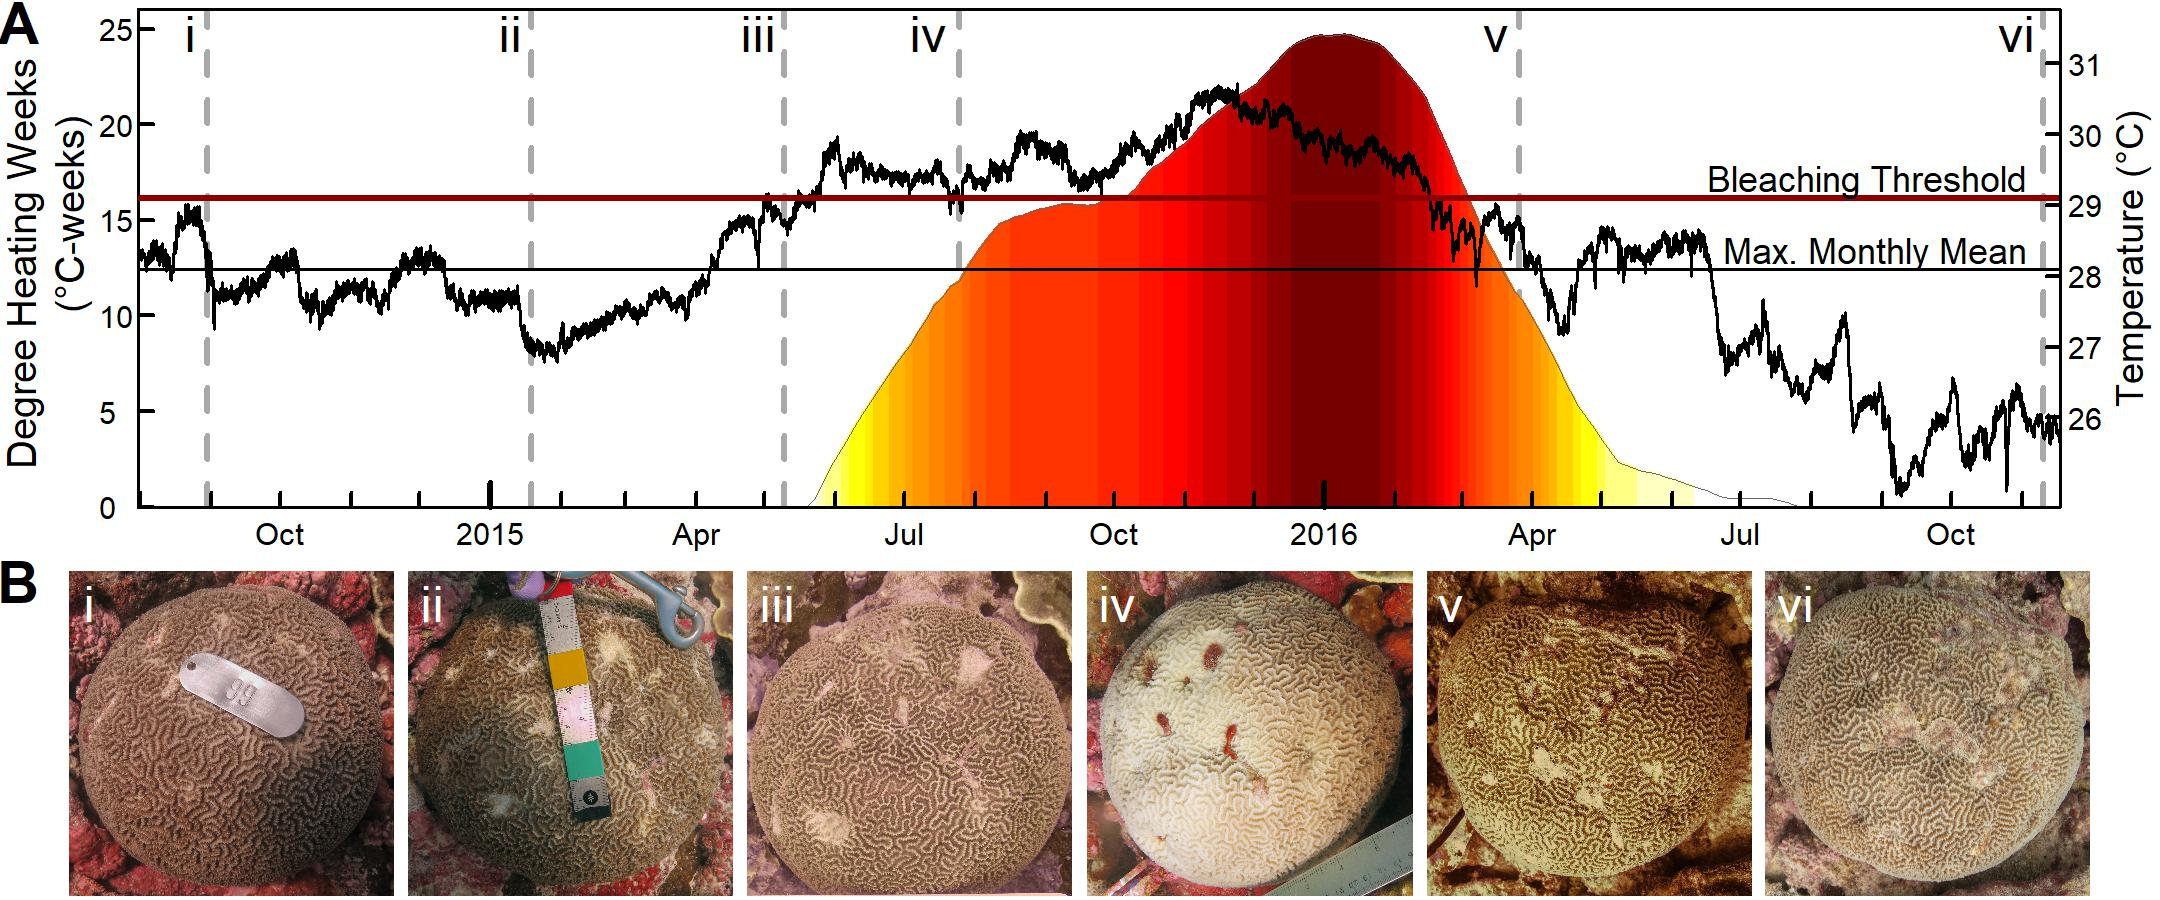
\includegraphics{../figures/Figure1.tiff}
\caption{Figure 1}
\end{figure}

The ``transient microbiome'' (of rare \emph{Symbiodinium} types)
assembled by environmental anomalies can undergo rapid changes (Putnam
et al 2017), providing symbiotic stochasticity which may build or weaken
a coral's capacity for resilience. While corals have been shown to
change symbiotic partners during a bleaching event (Chen et al 2005,
Jones et al 2008), there is often a quick return to pre-bleaching
\emph{Symbiodinium} communities after recovery (Thornhill 2005,
LaJeunesse et al 2010), and persistence of stress-related changes to
\emph{Symbiodinium} community structure may require sustained
environmental pressure (Baird et al 2007). Corals commonly host
background \emph{Symbiodinium} types in low levels (Correa et al 2009),
but sub-dominant \emph{Symbiodinium} communities are often unstable
(Coffroth et al 2010). The importance of rare \emph{Symbiodinium} types
is currently under debate, and these rare types may be commensal (pass
through coral's holobiont with no harm or gain for either partner),
parasitic (``cheaters'', or symbionts that take more than they give), or
mutualistic (symbionts which support host function) (Parkinson et al
2015). Some research suggests that low-abundance \emph{Symbiodinium}
types have minimal functional significance to corals (Lee et al 2016),
while other evidence supports the idea that the rare \emph{Symbiodinium}
biosphere is important for corals' response to climate change (Boulotte
et al 2016). However, shifts in \emph{Symbiodinium} community diversity
may still have a larger influence on coral resilience than the evolution
of symbiont thermal tolerance (Baskett et al 2010). In other systems,
other rare microbial species have been demonstrated to be
disproportionally important to maintaining functional processes during
environmental change (Shade et al 2014). We show that after two months
of heat stress, fully-bleached corals retained approximately the same
\emph{Symbiodinium} community as they had before the bleaching event.
This suggests that a wholesale breakdown of symbiosis occurred in
bleached corals during this event, indicating a lack of preferential
symbiont expulsion or exodus. Furthermore, we demonstrate that symbionts
present in even very low abundances can play a critical role in coral
survival and recovery. Some coral colonies recovered symbiosis with
\emph{Symbiodinium} types that were present in only a negligible amount
before the bleaching event.

Local protection is critical for coral symbiosis and survival. We show
that corals living at different levels of local human disturbance had
distinct symbiont communities that corresponded tightly to survivorship.
This is in contrast to a recent study which concluded that particulate
and dissolved nutrients do not reduce coral health at a colony scale
(Rocker et al 2017). However, there is increasing evidence for local
adaptation in corals (Howells et al 2012, Logan et al 2013, Dixon et al
2015). Our results suggest that some Kiritimati coral species may have
the capacity to experience evolutionary rescue, defined as adaptation at
a rate that allows an endangered population to survive the rate of
environmental change (Orr \& Unkless 2014, Carlson 2014). Our results
suggest that the capacity for evolutionary rescue is tangibly related to
local reef protection. Although massive bleaching events like this one
will likely continue to cause catastrophic damage to coral reefs
worldwide, mitigating local human disturbance can potentially help
protect some coral species against a modest amount of ocean warming.

\section*{Methods}\label{methods}
\addcontentsline{toc}{section}{Methods}

\emph{The Methods section should be written as concisely as possible but
should contain all elements necessary to allow interpretation and
replication of the results. As a guideline, Methods sections typically
do not exceed 3,000 words. Detailed descriptions of methods already
published should be avoided; a reference number can be provided to save
space, with any new addition or variation stated. The Methods section
should be subdivided by short bold headings referring to methods used
and we encourage the inclusion of specific subsections for statistics,
reagents and animal models. If further references are included in this
section, the numbering should continue from the end of the last
reference number in the rest of the paper and the list should accompany
the additional Methods at the end of the paper. The Methods section
cannot contain figures or tables (essential display items should be
included in the Extended Data).}

\subsection{Field Sampling}\label{field-sampling}

Kiritimati Atoll (Christmas Island), Kiribati is located in the Central
Equatorial Pacific (1.9N 157W), at the center of the El Niño 3.4 region
(a region which is used to quantify El Niño presence and strength).
During the 2015/2016 El Niño event, Kiritimati experienced 10 months of
sustained temperature stress, causing a mass bleaching and mortality
event (\textbf{???}).

\subsection{Temperature
quantification}\label{temperature-quantification}

Temperature loggers (Sea-Bird 56) were deployed around the island at
10-12m depth from 2011-2016 to measure \emph{in situ} thermal stress.

\subsection{Coral Tagging and
sampling}\label{coral-tagging-and-sampling}

In August/September 2014 colonies of \emph{Platygyra} sp. and
\emph{Favites pentagona} were tagged along a 60m transect at 10-12m
depth at 15 different sites around the atoll. A photo was taken of each
coral to record colony measurments and characteristics (i.e.~bleaching).
The tagged coral colonies were resampled twice more before
(January/February 2015, April/May 2015), once during (July 2015), and
once near the end (March 2016) of the El Niño warming. Some tagged coral
colonies were lost due to storm damage, and new coral colonies were
tagged to replenish the total number of surveyed colonies. Not all sites
were visited during all field seasons, and some site surveys were only
partially completed during some field seasons due to inclement weather
conditions.

Corals were sampled by\ldots{} processed like this\ldots{} Coral tissue
samples were preserved in Guanidinium buffer (50\% w/v guanidinium
isothiocyanate; 50 mM Tris pH 7.6; 10 µM EDTA; 4.2\% w/v sarkosyl; 2.1\%
v/v β-mercaptoethanol) and stored at 4 \emph{degrees} until extraction.

\subsection{Pre-processing and
sequencing}\label{pre-processing-and-sequencing}

DNA extraction was performed using a guanidinium-based extraction
protocol {[}14; Cunning2017-sc; Cunning2015-mt{]} with the modification
that the DNA pellet was washed with 70\% ethanol three times rather than
once.

Library Prep- Amy's method of library prep, include cleanup, Illumina
Sequencing information (barcodes, etc) for sequencing of ITS2 amplicons
(`itsD' and `its2rev2' primers from\textsuperscript{14} Illumina MiSeq
platform with 2×300 paired-end read chemistry. HIMB - Amy

ITS2 region - it's annoying, but it's the best we've got right now smith
et al 2017

A total of 289 samples were prepared for sequencing, and \emph{XXXX} of
these samples were successfully amplified, sequenced, and used in
downstream analyses.

\subsection{Bioinformatics}\label{bioinformatics}

We conducted quality filtering of raw reads (in .fastq format) first
using iu-filter-quality-bokulich implemented in Illumina-Utils {[}48;
Eren2013-yg{]}, followed by paired-end sequence merging via
iu-merge-pairs (also in Illumina-Utils, {[}Eren2013-yg{]}), with a
maximum mismatch of three bases between the forward and reverse reads.
After quality filtering, sequence processing and identification was
performed following all specifications of\textsuperscript{49}; chimeric
sequences were removed, primers were trimmed, sequences from each sample
were clustered independently at 97\% similarity using
UCLUST\textsuperscript{50} implemented in QIIME\textsuperscript{51} and
resulting OTUs were collapsed at 100\% identity across samples,
sequences were aligned using the Needleman-Wunsch global alignment
algorithm (Biostrings package,\textsuperscript{52}) in
R\textsuperscript{53}, and sequences were named using a reference
database.

The Phyloseq package\textsuperscript{54} in R was used to store and
analyze OTU tables, taxonomic information, and sample metadata. The
phyloseq object was filtered to remove OTUs observed \textless{}10
times, which removed more than half of observed otus (n=\emph{83} OTUs
removed and n=\emph{81} kept, including n=\emph{10} doubletons). The
phyloseq object was further filtered to remove samples with very low
sequence abundance (\textless{}200 sequences, n=\emph{27} samples
removed and n=\emph{262} kept).

In \emph{262} coral samples, we found XXXX sequences after quality
filtering. \emph{clade abundances here}

\subsection{Statistical Analysis}\label{statistical-analysis}

Code will be avaible on git hub

\section*{References}\label{references}
\addcontentsline{toc}{section}{References}

\hypertarget{refs}{}
\hypertarget{ref-Sampayo2016-vd}{}
1. Sampayo, E. M. \emph{et al.} Coral symbioses under prolonged
environmental change: Living near tolerance range limits. \emph{Sci.
Rep.} \textbf{6,} 36271 (2016).

\hypertarget{ref-Hughes2003-aj}{}
2. Hughes, T. P. \emph{et al.} Climate change, human impacts, and the
resilience of coral reefs. \emph{Science} \textbf{301,} 929--933 (2003).

\hypertarget{ref-Hoegh-Guldberg2007-fh}{}
3. Hoegh-Guldberg, O. \emph{et al.} Coral reefs under rapid climate
change and ocean acidification. \emph{Science} \textbf{318,} 1737--1742
(2007).

\hypertarget{ref-Baker2008-ky}{}
4. Baker, A. C., Glynn, P. W. \& Riegl, B. Climate change and coral reef
bleaching: An ecological assessment of long-term impacts, recovery
trends and future outlook. \emph{Estuar. Coast. Shelf Sci.} \textbf{80,}
435--471 (2008).

\hypertarget{ref-Muscatine1977-pn}{}
5. Muscatine, L. \& Porter, J. W. Reef corals: Mutualistic symbioses
adapted to Nutrient-Poor environments. \emph{Bioscience} \textbf{27,}
454--460 (1977).

\hypertarget{ref-Rowan1992-lg}{}
6. Rowan, R. \& Powers, D. A. Ribosomal RNA sequences and the diversity
of symbiotic dinoflagellates (zooxanthellae). \emph{Proc. Natl. Acad.
Sci. U. S. A.} \textbf{89,} 3639--3643 (1992).

\hypertarget{ref-Baker2003-ks}{}
7. Baker, A. C. Flexibility and specificity in Coral-Algal symbiosis:
Diversity, ecology, and biogeography of symbiodinium. \emph{Annu. Rev.
Ecol. Evol. Syst.} \textbf{34,} 661--689 (2003).

\hypertarget{ref-Little2004-tm}{}
8. Little, A. F., Oppen, M. J. H. van \& Willis, B. L. Flexibility in
algal endosymbioses shapes growth in reef corals. \emph{Science}
\textbf{304,} 1492--1494 (2004).

\hypertarget{ref-Thornhill2006-cs}{}
9. Thornhill, D. J., LaJeunesse, T. C., Kemp, D. W., Fitt, W. K. \&
Schmidt, G. W. Multi-year, seasonal genotypic surveys of coral-algal
symbioses reveal prevalent stability or post-bleaching reversion.
\emph{Mar. Biol.} \textbf{148,} 711--722 (2006).

\hypertarget{ref-Thornhill2009-jh}{}
10. Thornhill, D. J., Xiang, Y., Fitt, W. K. \& Santos, S. R. Reef
endemism, host specificity and temporal stability in populations of
symbiotic dinoflagellates from two ecologically dominant caribbean
corals. \emph{PLoS One} \textbf{4,} e6262 (2009).

\hypertarget{ref-Lesser2013-dj}{}
11. Lesser, M. P., Stat, M. \& Gates, R. D. The endosymbiotic
dinoflagellates (symbiodinium sp.) of corals are parasites and
mutualists. \emph{Coral Reefs} \textbf{32,} 603--611 (2013).

\hypertarget{ref-Brown1997-mf}{}
12. Brown, B. E. Coral bleaching: Causes and consequences. \emph{Coral
Reefs} \textbf{16,} S129--S138 (1997).

\hypertarget{ref-Douglas2003-nr}{}
13. Douglas, A. E. Coral bleaching----how and why? \emph{Mar. Pollut.
Bull.} \textbf{46,} 385--392 (2003).

\hypertarget{ref-Stat2009-qq}{}
14. Stat, M., Loh, W. K. W., LaJeunesse, T. C., Hoegh-Guldberg, O. \&
Carter, D. A. Stability of coral--endosymbiont associations during and
after a thermal stress event in the southern great barrier reef.
\emph{Coral Reefs} \textbf{28,} 709--713 (2009).

\hypertarget{ref-Heron2016-am}{}
15. Heron, S. F., Maynard, J. A., Hooidonk, R. van \& Eakin, C. M.
Warming trends and bleaching stress of the world's coral reefs
1985-2012. \emph{Sci. Rep.} \textbf{6,} 38402 (2016).

\hypertarget{ref-Van_Oppen2006-qf}{}
16. Oppen, M. J. H. van \& Gates, R. D. Conservation genetics and the
resilience of reef-building corals. \emph{Mol. Ecol.} \textbf{15,}
3863--3883 (2006).

\hypertarget{ref-Gates2011-zy}{}
17. Gates, R. D. \& Ainsworth, T. D. The nature and taxonomic
composition of coral symbiomes as drivers of performance limits in
scleractinian corals. \emph{J. Exp. Mar. Bio. Ecol.} \textbf{408,}
94--101 (2011).

\hypertarget{ref-Van2005-di}{}
18. van., M. J., Mahiny, A. J. \& Done, T. J. Geographic distribution of
zooxanthella types in three coral species on the great barrier reef
sampled after the 2002 bleaching event. \emph{Coral Reefs} \textbf{24,}
482--487 (2005).

\hypertarget{ref-Franklin2012-sz}{}
19. Franklin, E. C., Stat, M., Pochon, X., Putnam, H. M. \& Gates, R. D.
GeoSymbio: A hybrid, cloud-based web application of global geospatial
bioinformatics and ecoinformatics for symbiodinium--host symbioses.
\emph{Mol. Ecol. Resour.} \textbf{12,} 369--373 (2012).

\hypertarget{ref-Tonk2013-pf}{}
20. Tonk, L., Bongaerts, P., Sampayo, E. M. \& Hoegh-Guldberg, O.
SymbioGBR: A web-based database of symbiodinium associated with
cnidarian hosts on the great barrier reef. \emph{BMC Ecol.} \textbf{13,}
7 (2013).

\hypertarget{ref-Stat2012-gw}{}
21. Stat, M. \emph{et al.} 1 molecular delineation of species in the
coral holobiont. \emph{Adv. Mar. Biol.} \textbf{63,} (2012).

\hypertarget{ref-LaJeunesse2001-hf}{}
22. LaJeunesse, T. C. INVESTIGATING THE BIODIVERSITY, ECOLOGY, AND
PHYLOGENY OF ENDOSYMBIOTIC DINOFLAGELLATES IN THE GENUS SYMBIODINIUM
USING THE ITS REGION: IN SEARCH OF a `SPECIES' LEVEL MARKER. \emph{J.
Phycol.} \textbf{37,} 866--880 (2001).

\hypertarget{ref-Pochon2010-jm}{}
23. Pochon, X. \& Gates, R. D. A new symbiodinium clade (dinophyceae)
from soritid foraminifera in hawai'i. \emph{Mol. Phylogenet. Evol.}
\textbf{56,} 492--497 (2010).

\hypertarget{ref-Fabina2012-mm}{}
24. Fabina, N. S., Putnam, H. M., Franklin, E. C., Stat, M. \& Gates, R.
D. Transmission mode predicts specificity and interaction patterns in
coral-symbiodinium networks. \emph{PLoS One} \textbf{7,} e44970 (2012).

\hypertarget{ref-Fitt2000-ex}{}
25. Fitt, W. K., McFarland, F. K., Warner, M. E. \& Chilcoat, G. C.
Seasonal patterns of tissue biomass and densities of symbiotic
dinoflagellates in reef corals and relation to coral bleaching.
\emph{Limnol. Oceanogr.} \textbf{45,} 677--685 (2000).

\hypertarget{ref-Cunning2012-um}{}
26. Cunning, R. \& Baker, A. C. Excess algal symbionts increase the
susceptibility of reef corals to bleaching. \emph{Nat. Clim. Chang.}
\textbf{3,} 259--262 (2012).

\hypertarget{ref-Stat2008-hk}{}
27. Stat, M., Morris, E. \& Gates, R. D. Functional diversity in
coral--dinoflagellate symbiosis. \emph{Proceedings of the National
Academy of Sciences} \textbf{105,} 9256--9261 (2008).

\hypertarget{ref-Quigley2014-zj}{}
28. Quigley, K. M. \emph{et al.} Deep-sequencing method for quantifying
background abundances of symbiodinium types: Exploring the rare
symbiodinium biosphere in reef-building corals. \emph{PLoS One}
\textbf{9,} e94297 (2014).

\hypertarget{ref-Arif2014-kx}{}
29. Arif, C. \emph{et al.} Assessing symbiodinium diversity in
scleractinian corals via next-generation sequencing-based genotyping of
the ITS2 rDNA region. \emph{Mol. Ecol.} \textbf{23,} 4418--4433 (2014).

\hypertarget{ref-Green2014-az}{}
30. Green, E. A., Davies, S. W., Matz, M. V. \& Medina, M. Quantifying
cryptic symbiodinium diversity within orbicella faveolata and orbicella
franksi at the flower garden banks, gulf of mexico. \emph{PeerJ}
\textbf{2,} e386 (2014).

\hypertarget{ref-Edmunds_undated-fd}{}
31. Edmunds, P. J. \emph{et al.} Long-term changes in symbiodinium
communities in orbicella annularis in st. john, US virgin islands.

\hypertarget{ref-Putnam2012-om}{}
32. Putnam, H. M., Stat, M., Pochon, X. \& Gates, R. D. Endosymbiotic
flexibility associates with environmental sensitivity in scleractinian
corals. \emph{Proc. Biol. Sci.} \textbf{279,} 4352--4361 (2012).

\hypertarget{ref-Buddemeier2004-se}{}
33. Buddemeier, R. W., Baker, A. C., Fautin, D. G. \& Jacobs, J. R. The
adaptive hypothesis of bleaching. \emph{Coral health and disease}
\textbf{427444,} (2004).

\hypertarget{ref-Buddemeier1993-sx}{}
34. Buddemeier, R. W. \& Fautin, D. G. Coral bleaching as an adaptive
mechanism. \emph{Bioscience} \textbf{43,} 320--326 (1993).

\hypertarget{ref-Baker2001-vc}{}
35. Baker, A. C. Ecosystems: Reef corals bleach to survive change.
\emph{Nature} \textbf{411,} 765--766 (2001).

\hypertarget{ref-Boulotte2016-dy}{}
36. Boulotte, N. M. \emph{et al.} Exploring the symbiodinium rare
biosphere provides evidence for symbiont switching in reef-building
corals. \emph{ISME J.} \textbf{10,} 2693--2701 (2016).

\hypertarget{ref-Kemp2014-xj}{}
37. Kemp, D. W., Hernandez-Pech, X., Iglesias-Prieto, R., Fitt, W. K. \&
Schmidt, G. W. Community dynamics and physiology of symbiodinium spp.
before, during, and after a coral bleaching event. \emph{Limnol.
Oceanogr.} \textbf{59,} 788--797 (2014).

\hypertarget{ref-Stat2010-zg}{}
38. Stat, M. \& Gates, R. D. Clade D symbiodinium in scleractinian
corals: A `nugget' of hope, a selfish opportunist, an ominous sign, or
all of the above? \emph{J. Mar. Biol.} \textbf{2011,} (2010).

\hypertarget{ref-Berkelmans2006-rf}{}
39. Berkelmans, R. \& Oppen, M. J. H. van. The role of zooxanthellae in
the thermal tolerance of corals: A 'nugget of hope' for coral reefs in
an era of climate change. \emph{Proc. Biol. Sci.} \textbf{273,}
2305--2312 (2006).

\hypertarget{ref-Mieog2007-yy}{}
40. Mieog, J. C. \emph{et al.} Real-time PCR reveals a high incidence of
symbiodinium clade D at low levels in four scleractinian corals across
the great barrier reef: Implications for symbiont shuffling. \emph{Coral
Reefs} \textbf{26,} 449 (2007).

\hypertarget{ref-Silverstein2012-tm}{}
41. Silverstein, R. N., Correa, A. M. S. \& Baker, A. C. Specificity is
rarely absolute in coral--algal symbiosis: Implications for coral
response to climate change. \emph{Proceedings of the Royal Society of
London B: Biological Sciences} \textbf{279,} 2609--2618 (2012).

\hypertarget{ref-Stat2013-qp}{}
42. Stat, M. \emph{et al.} The distribution of the thermally tolerant
symbiont lineage (symbiodinium clade d) in corals from hawaii:
Correlations with host and the history of ocean thermal stress.
\emph{Ecol. Evol.} \textbf{3,} 1317--1329 (2013).

\hypertarget{ref-Jones2011-nf}{}
43. Jones, A. M. \& Berkelmans, R. Tradeoffs to thermal acclimation:
Energetics and reproduction of a reef coral with heat tolerant
symbiodinium Type-D. \emph{J. Mar. Biol.} \textbf{2011,} (2011).

\hypertarget{ref-Sampayo2008-tw}{}
44. Sampayo, E. M., Ridgway, T., Bongaerts, P. \& Hoegh-Guldberg, O.
Bleaching susceptibility and mortality of corals are determined by
fine-scale differences in symbiont type. \emph{Proceedings of the
National Academy of Sciences} \textbf{105,} 10444--10449 (2008).

\hypertarget{ref-Gates1992-ew}{}
45. Gates, R. D., Baghdasarian, G. \& Muscatine, L. Temperature stress
causes host cell detachment in symbiotic cnidarians: Implications for
coral bleaching. \emph{Biol. Bull.} \textbf{182,} 324--332 (1992).

\hypertarget{ref-Hoegh-Guldberg1999-rb}{}
46. Hoegh-Guldberg, O. Climate change, coral bleaching and the future of
the world's coral reefs. \emph{Mar. Freshwater Res.} \textbf{50,}
839--866 (1999).

\hypertarget{ref-Hoegh-Guldberg2011-sl}{}
47. Hoegh-Guldberg, O. Coral reef ecosystems and anthropogenic climate
change. \emph{Regional Environ. Change} \textbf{11,} 215--227 (2011).

\hypertarget{ref-Bokulich2013-cm}{}
48. Bokulich, N. A. \emph{et al.} Quality-filtering vastly improves
diversity estimates from illumina amplicon sequencing. \emph{Nat.
Methods} \textbf{10,} 57--59 (2013).

\hypertarget{ref-Cunning2017-sc}{}
49. Cunning, R., Gates, R. D. \& Edmunds, P. J. Using high-throughput
sequencing of ITS2 to describe symbiodinium metacommunities in st. john,
US virgin islands. \emph{PeerJ} \textbf{5,} e3472 (2017).

\hypertarget{ref-Edgar2010-zl}{}
50. Edgar, R. C. Search and clustering orders of magnitude faster than
BLAST. \emph{Bioinformatics} \textbf{26,} 2460--2461 (2010).

\hypertarget{ref-Caporaso2010-yl}{}
51. Caporaso, J. G. \emph{et al.} QIIME allows analysis of
high-throughput community sequencing data. \emph{Nat. Methods}
\textbf{7,} 335--336 (2010).

\hypertarget{ref-Pages2017-ie}{}
52. Pagès, H., Aboyoun, P., Gentleman, R. \& DebRoy, S. Biostrings:
String objects representing biological sequences, and matching
algorithms. (2017).

\hypertarget{ref-R_Development_Core_Team2008-sp}{}
53. R Development Core Team. R: A language and environment for
statistical computing. (2008).

\hypertarget{ref-McMurdie2013-hf}{}
54. McMurdie, P. J. \& Holmes, S. Phyloseq: An R package for
reproducible interactive analysis and graphics of microbiome census
data. \emph{PLoS One} \textbf{8,} e61217 (2013).


\end{document}
